\documentclass[12pt,a4paper]{article}

\usepackage[utf8]{inputenc}
\usepackage[french]{babel}
\usepackage[T1]{fontenc}
\usepackage[margin=3.5cm]{geometry}
\usepackage{graphicx}
\usepackage{makeidx}
\usepackage{url}
\usepackage{caption}
\usepackage{subcaption}
\usepackage{enumerate}
\usepackage{enumitem}
\usepackage{ifthen}
\usepackage{amssymb}
\usepackage{dsfont}
\usepackage{multicol}
\usepackage[hidelinks]{hyperref}
\usepackage{amsmath}
\usepackage{multirow}
\usepackage{pgfplotstable}
\usepackage{booktabs}
\usepackage{csvsimple}
\usepackage[toc,page]{appendix} 

\newcommand{\figref}[1]{Figure~\ref{fig:#1}}
\newcommand{\tabref}[1]{Table~\ref{tab:#1}}
\newcommand{\secref}[1]{Section~\ref{sec:#1}}
\newcommand{\alref}[1]{Algorithm~\ref{alg:#1}}
\newcommand{\lstref}[1]{Listing~\ref{lst:#1}}
\renewcommand{\appendixtocname}{Annexes} 
\renewcommand{\appendixpagename}{Annexes} 


\title{\vspace{4cm}\textbf{Impact of Renaming on Software Change Metrics}\vspace{3cm}}

\author{
Pierre Chanson\\\\
Mémoire de stage de Master2\\
Encadrants: Jean-Rémy Falleri et Matthieu Foucault\\\\
LaBRI, UMR 5800\\
F-33400, Talence, France\\\\
\texttt{Email: pierre.chanson@etu.u-bordeaux.fr,}\and
\texttt{\{falleri,mfoucault\}@labri.fr}\\
}


\begin{document}

\begin{figure}[t]
\center

\includegraphics[scale=0.25]{data/figures/UnivBordeaux.jpg}
\end{figure}
\maketitle
\newpage
\tableofcontents
\newpage
\section{Introduction}
\label{sec:intro}

L'accès aux dépôts logiciels a rendu possible de nombreux travaux de recherche sur l'évolution logicielle. Plus particulièrement, les dépôts de code source gérés par des outils de contrôle de versions (Version Control System, VCS, comme SVN, Mercurial ou encore Git) contiennent l'historique de construction d'un logiciel. Principalement dans le domaine du ``Reverse Engineering'', la compréhension des choix des développeurs lors de la création d'un logiciel, des études se basent sur l'analyse de ces historiques. Ces études entrent dans le cadre des études ``MSR'' (Minning Software Repository). De même, la prédiction de bugs, un des défis connus du Génie Logiciel dont le but est de prédire le nombre de bugs et leur localisation dans la prochaine version d'un logiciel, utilise des informations contenu dans l'historique d'un projet. Cette étude se base sur les métriques de procédés comme prédicateurs de bugs. Les métriques de procédés se concentrent sur l'évolution d'un logiciel et mesurent les modifications subies par les entités d'un code source durant leur cycle de vie. L'hypothèse principale étant que la manière dont les entités du code ont changé a un impact majeur sur la qualité de leur prédiction de bugs.\\
Or au cours de son histoire, un fichier peut être renommé et/ou déplacé dans un autre dossier du projet.\\
Théoriquement, si le renommage d'un fichier à un moment donné de son histoire n'est pas pris en compte, le calcul d'une métrique de procédé sur ce fichier sera faussé. En effet, si on identifie le fichier par son nom, on perdra les informations récoltées avant le renommage. Par ailleurs on peut penser que le refactoring, dont le renommage de fichiers, est très présent dans le développement des logiciels à succès d'aujourd'hui. En pratique, nous n'avons pas de chiffres pour le montrer.\\ 
Dans un premier temps nous effectuerons une étude de l'existant sur les méthodes utilisées pour détecter le refactoring, les logiciels qui ont été étudié, les métriques de procédés ainsi que les VCS. Puis nous choisirons un ensemble de projets cohérent pour faire nos propres expérimentations, nous définirons un niveau de granularité et nous ferons une analyse manuelle des projets choisis pour récupérer les renommages réels. Par la suite, nous définirons un modèle et nous utiliserons un outil pour récupérer les renommages. Enfin, nous définirons comment calculer certaines métriques de procédés et mesurerons l'impact du renommage. Les résultats de nos expérimentations amèneront à une publication dans la conférence ICSME 2014.\\


\section{Etat de l'art}
\label{sec:etat_de_lart}

\subsection{Evolution logiciel et refactoring}

\subsection{Métriques de procédés et évolution logiciel}

\begin{figure}[t]
	\centering
	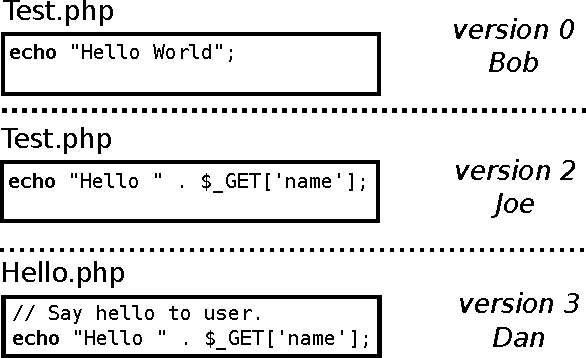
\includegraphics[width=0.8\linewidth,keepaspectratio]{data/figures/example.pdf}
	\caption{Example of a project history. The project is composed of only one file \texttt{Test.php} which is renamed to \texttt{Hello.php} in the last version.}
	\label{fig:example}
\end{figure}

\subsection{Les outils}


\begin{table}
\centering
\begin{tabular}{rccc}
\toprule
 & \multicolumn{3}{c}{Renaming handling}\\
\cmidrule{2-4}
& & \multicolumn{2}{c}{Automatic}\\
\cmidrule{3-4}
Tool & Manual & Standard & Optional\\
\midrule
CVS & & &\\
Subversion & $\times$ & &\\
Mercurial & $\times$ & & $\times$\\
Git & & & $\times$\\
\bottomrule
\end{tabular}
\caption{Handling of renaming of the main VCS tools.}
\label{tab:vcs}
\end{table}

\section{Problématique}
\label{sec:problematique}
Nous n'avons pas trouvé d'études traitant le renommage. Ces études ont elles volontairement ou non omis le renommage ? \\
La problématique qui se pose est donc la suivante:\\
 \textbf{Quelle est la quantité de renommages ou déplacements de fichiers dans les projets ? Où interviennent-ils ? Ont-ils un réel impact sur les métriques de procédés ?} \\

\section{Première analyse à fine granularité}
\label{sec:analyse_fin_grain}

Le premier travail réalisé durant le stage a consisté à réaliser une analyse manuelle des renommages dans les VCS. Nous avons sélectionné 100 commits de manière aléatoire dans un projet et étudié le renommage d'entités dans ces commits.

Nous avons choisi Hibernate-ORM, un projet open-source connue et assez gros, $750000$ LOC, avec suffisamment de développeurs, $138$, et en JAVA afin de pouvoir différencier les renommages à différents niveaux de granularité.\\
Nous avons pris $4$ niveaux de granularité: Dossier, fichier, classe et fonction. Nous avons défini l'identité d'une entité de code source par son path plus un type. \\\\
dossier = folder/folder/ | FOLDER\\
fichier = folder/folder/file | FILE\\
classe = folder/folder/file | CLASS\\
fonction = folder/folder/file\#func(types) | FUNC\\
classe interne = folder/folder/file\$class | CLASS\\

Nous nous sommes ensuite intéressés à la localisation des renommages. Sont-ils plus proches des releases majeurs que des releases mineurs ? Nous nous sommes aussi demandé si Git détectait ces renommages au niveau des fichiers, et si cela pouvait être un indicateur pour tous les changements d'identité.

Nous avons donc décidé d'utiliser à partir de maintenant la détection de renommages de Git, afin de couvrir un grand nombre de commits dans plusieurs projets et plusieurs langages de programmation et donc nous fixer à un seul niveau de granularité, les fichiers.\\

\section{Un modèle}
\label{sec:model}


 


\section{Un ensemble de projet}
\label{sec:ensemble_projet}
Nous avons donc du sélectionner un ensemble de projets sur lesquels effectuer nos expérimentations qui respectent le modèle définit. Des projets open-source, conséquents et connues de la communauté MSR. Nous avons un ensemble de projets utilisé par l'equipe de Génie Logiciel au LaBRI qui respectent le modèle avec des branches de maintenances identifiés. Les $5$ projets qui sont donnés \tabref{projects} nous fournissent un corpus pour notre prochaine expérience avec differents langages de programmation, un nombre de lignes de code ainsi qu'un nombre de développeurs dans la moyenne jusqu'à évelé par rapport aux projets open source utilisés par la communautée. Les $5$ projets sont gérés sur Git afin de profiter du détectage automatique des renommages (section). \\
De plus, il faut noter que nous avons choisis d'exclure tout les fichiers qui ne sont pas du code source du corpus étant donné que les métriques de procédés sont habituellement uniquement calculé sur ces fichiers.  \\

\begin{table*}[t]
\centering
\begin{tabular}{rcccc}
\toprule
Project & Main language & Size (LoC) & Number of developers & URL\\
\midrule
Jenkins & Java & 200851 & 454 & \url{github.com/jenkinsci/jenkins} \\
JQuery & JavaScript & 41656 & 223 & \url{github.com/jquery/jquery} \\
PHPUnit & PHP & 21799 & 152 & \url{github.com/sebastianbergmann/phpunit}\\
Pyramid & Python & 38726 & 205 & \url{github.com/Pylons/pyramid} \\
Rails & Ruby & 181002 & 2767 & \url{github.com/rails/rails}\\
\bottomrule
\end{tabular}
\caption{Our corpus of software projects.}
\label{tab:projects}
\end{table*}

\section{Analyse à gros grain}
\label{sec:analyse_gros_grain}

\subsection{Première experience}
L'objectif de notre première expérience est de mieux comprendre le renommage d'entités. En particulier, d'observer quand les renommages apparaissent et en quelle quantité. Nous avons donc analysé chaque période comme décrites précédemment sur chaque projet de notre corpus. Nous comptons donc sur la détection automatique de renommage de Git et l'utilisons dans notre outil développé en Ruby pour obtenir nos chiffres (détails dans la section résultats). (TODO pourquoi Ruby ?) Nous suivons ces trois étapes entre chaque période:
\begin{enumerate}
\item On liste les fichiers existant à la fin de la période.
\item Pour chacun de ces fichiers, on extrait sa séquence de modification durant la période en activant la détection de renommage (commande \texttt{git log -M})
\item On calcule à partir des informations receuillies. Par exemple le pourcentage de fichiers $\%F_{R}$ qui ont été renommés au moins une fois durant la période.
\end{enumerate}
\medskip
Plus précisément voici le déroulement général de notre outil:

Avant tout nous avons besoin de la liste des tags de release trié dans l'ordre chronologique. Cette partie ne peut être automatisé en raison des conventions de nom de tags différentes entre chaque projets. Par exemple: 
\begin{itemize}
\item PHPunit: \texttt{3.5.0, 3.6.0} etc.
\item Pyramid: \texttt{1.0, 1.1} etc.
\item Jenkins: \texttt{jenkins-1\_400, jenkins-1\_410} etc.
\item Rails: \texttt{v2.0.0, v2.1.0} etc.
\end{itemize}
\medskip
Enfin voici le déroulement du processus :

Nous parcourons les branches distantes (\texttt{remotes}) du dépôt Git du projet. Toute les branches sont considérés comme branche de maintenance, sauf la branche \texttt{master}. La plus part du temps, les branches spécifiques de maintenance contiennent ``-stable'' dans leur nom, mais si une branche est listée ici, cela veut dire que la tête de branche, c'est à dire sa dernière version, est séparée et n'est pas joignable de la branche \texttt{master}. C'est donc une branche de maintenance depuis son dernier \texttt{merge} avec master, c'est à dire depuis leur dernière fusion. Il est laissé à la discrétion de chacun d'éliminer les branches qui ne sont pas spécifiquement de maintenance au préalable, mais dans nos expériences, ces branches n'ont pas faussé notre étude. En général les branches présentes sur le dépôt qui ne sont ni \texttt{master} ni de maintenance ne contennaient peux ou pas de \texttt{commits}.

La branche \texttt{origin/master} contient la partie initiale (init) et la partie de développement (dev).\\  
Le travail est donc réalisé sur: 
\begin{itemize}
\item Les branches de maintenance
\item La branche \texttt{origin/master}
\end{itemize}
\medskip
Si la branche est \texttt{origin/master}, le travail est divisé encore dans les périodes:
\begin{itemize}
\item Du premier commit(inclue) jusqu'au premier tag de release.
\item Du premier jusqu'au dernier tag (une release après l'autre forme une période).*
\end{itemize}
\medskip

(* nous ne considérons pas la période du dernier tag jusqu'à la tête de la branche master, car la release n'étant pas terminé, le nombre de commit ne sera pas de la taille d'une release normale et les chiffres obtenus sur cette partie ne seront donc pas pertinants)

Ainsi, pour chacune de nos trois conditions, maintenance(maint), période initiale(init) et releases(dev) qui formes l'ensemble des périodes que nous analysons, nous allons générer le \texttt{log}. Le \texttt{log} donné par la commande \texttt{git log} contient l'ensemble des \texttt{commits} dans nos périodes avec toute les informations nécessaires pour chacun d'eux.

La majeure partie du travail réalisé se situe sur ces \texttt{log}. Nous avons choisis de travailler sur un \texttt{log} général plutôt qu'en récupérant l'historique de chaque fichier (avec l'option \texttt{``--follow''}) l'un après l'autre pour des raisons de performances. Particulièrement sur les gros projets tels que Rails ou Jenkins, cette dernière technique n'est presque pas réalisable. De plus elle n'est réalisable que sur les fichiers présent à la tête de la branche et pas à partir d'une version antérieure, ce qui impliquerais un travail supplémentaire pour configurer le dépôt à chaque release sur la branche \texttt{master}.\\

Nous listons les fichiers existants à la fin de chaque période. Dans notre expérience nous écartons les fichiers qui ne sont pas du code source. 
Enfin l'algorithme principal, qui parcours des informations contenus par les \texttt{log} dans l'ordre chronologique, va nous permettre de suivre les renommages et les modifications et ainsi reconstruire l'histoire des fichiers. Un renommage typique ressemble à \texttt{``rename bob/\{henry $\Rightarrow$ josef\}/george.py (86\%)''}. Si \texttt{''bob/henry/george.py''} à été enregistré au préalable par notre algorithme nous suivrons maintenant \texttt{''bob/josef/george.py''} à la place. Il y a de nombreux cas particuliers à prendre en compte et de nombreuses applications possible par rapport aux informations récupérés ainsi. On peut choisir de ne considérer que le dernier nom d'un fichier par exemple ou stocker tout ses noms précédents. on élimine finalement tout les fichiers qui ne sont pas dans notre liste de établie au préalable.\\

À notre connaissance, il n'existe pas d'évaluation empirique de l'algorithme utilisé par Git pour détecter les renommages. Néanmoins, nous procédons à une évaluation manuelle de son comportement dans la partie conclusion et nous n'avons pas noté de faux positif sur 100 renommages aléatoire récupérés par notre outil.(TODO partie vérif?)\\

\subsection{Deuxième expérience}

\subsubsection{Calcul des métriques}
Un gestionnaire de versions (VCS) offre plusieurs moyens de calculer les métriques de procédés car il stocke les informations sur les entités modifiées à chaque nouvelle version, l'auteur de ces modifications, la date, etc. De plus, il permet la récupération du contenu de chaque entité et de l'ensemble d'un projet à une version donnée. Pour calculer ces métriques, il est donc possible d'analyser chaque entité modifiée lors d'une période puis de garder uniquement les entités toujours présentes à la dernière version de notre période.

Par ailleurs, il faut noter qu'un VCS identifie une entité par son chemin $+$ nom de fichier. On en déduit qu'un renommage du fichier ou d'un dossier, aura un impact sur le calcul des métriques. Pour expliquer cet impact, il est présenté un exemple d'historique d'un logiciel figure 2. Ce projet ne contient qu'une entité, Test.php, qui est renommé en Hello.php dans la dernière version. Dans cet exemple nous calculons le nombre de développeurs (NoD) entre la version 1 et 3.

Le NoD d'une entité de code source au cours d'une période de son histoire correspond au nombre de développeurs ayant été identifiés comme auteurs d'une modification sur l'entité pendant la période donnée.\\

\begin{figure}[t]
	\centering
	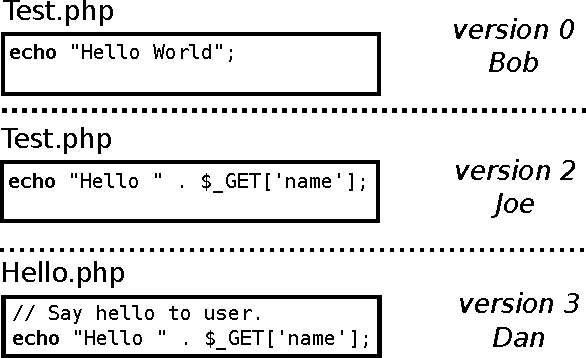
\includegraphics[width=0.8\linewidth,keepaspectratio]{data/figures/example.pdf}
	\caption{Exemple d'un historique de projet. Le projet est composé d'un seul fichier \texttt{Test.php} qui est renommé en \texttt{Hello.php} dans la dernière version.}
	\label{fig:example}
\end{figure}
En ne prenant pas en compte le renommage, la dernière version ne contient qu'une entité. C'est donc cette entité uniquement qui sera considérée. De plus, l'identité exacte de cette entité n'apparaît que lors de la version 3. Le calcul des métriques est donc trivial, NoD$ = 1$.

Par ailleurs, en prenant en compte le fait que ce fichier a été renommé, il y a trois versions à considérer en ce qui concerne l'entité. Le premier nom du fichier était Test.php. Ce fichier a un premier auteur lors de la version 1 puis un deuxième à la version 2. Le fichier est ensuite renommé en Hello.php par un troisième auteur. Le NoD est donc de 3.\\

Nous avons choisi de nous concentrer sur les trois métriques de procédés identifiés plus tôt pour mesurer l'impact du renommage. En utilisant des scripts Ruby pour mesurer les métriques sur nos projets, voici plus précisément notre procédure: 

\begin{enumerate}
\item  Nous récupérons d'abord la dernière version du projet pour obtenir les entités existantes à la fin de la période considérée. On note $A$ cet ensemble d'entités.
\item Toujours grâce aux commandes git, nous récupérons toutes les modifications effectuées durant la période. On note $C$ l'ensemble des modifications dans l'ordre chronologique.
\item  Troisièmement, nous parcourons cet ensemble de modifications en commençant par la plus ancienne ($c_0 \in C$) jusqu'à la plus récente ($c_n \in C$) dans le but de calculer les métriques de procédés pour chaque entité.
\end{enumerate}

 On note $\mu_{a}^{M}$ la valeur de la métrique $M$ pour l'entité $a$. Ensuite nous calculons les métriques comme suivant (on note $c_i$ la modification courante lors du parcours):

\begin{description}
	\item[NoD] (nombre de développeurs) Pour chaque entité $a$ pointé par $c_i$ qui appartient aussi à $A$ ($a \in A$), on ajoute à $\mu_{a}^{NoD}$ le nombre d'auteurs qui ont effectué les modifications $c_i$ et qui ont modifiés $a$ pour la première fois dans la période.
	\item[NoC] (nombre de modifications) Pour chaque entité $a$ pointé par $c_i$ qui appartient aussi à $A$ ($a \in A$), on ajoute $1$ à $\mu_{a}^{C}$ tels que $c_i$ indique qu'une nouvelle modification a été effectuée.
	\item[CC] (Code Churn) Pour chaque entité $a$ pointé par $c_i$ qui appartient aussi à $A$ ($a \in A$), on vérifie d'abord que la modification n'est pas une creation d'entité. Si c'est le cas celà veut dire que l'entité a été créée durant la période, donc on initialise son $\mu_{a}^{CC}$ à son nombre de lignes. Ensuite au prochain $c_j$ qui cible $a$ dans la période avec ($i < j$), on compare les deux versions et on ajoute à $\mu_{a}^{CC}$ le nombre de lignes ajoutées ou suprimées.
\end{description}

\subsubsection{Calcul de corrélation}

L'objectif de la deuxième expérience est de voir si le renommage peut biaiser significativement les valeurs des métriques de procédés décrites ci-dessus. Pour ça, nous effectuons une analyse dans le pire des cas.(TODO expliquer ?) On sélectionne la période de nos projets qui a la plus grande valeur de fichiers renommés en excluant la période initiale qui n'est généralement pas observée dans les études. Nous calculons ensuite les trois métriques avec et sans le renommage de fichiers pris en compte, puis nous calculons la corrélation de coefficient de Spearman entre les métriques avec et sans la détection de renommage. Un coefficient élevé, proche de $1$, indiquera que les métriques avec et sans détection de renommage sont très similaires alors qu'un coefficient plus petit, 0.5 et moins, indiquera que les métriques avec et sans détection de renommage sont très différentes.\\ 

\section{Resultats}
\label{sec:resultats}

\subsection{resultats première expérience}

\subsection{resultats deuxième expérience}

\section{Conclusion}
\label{sec:conclusion}

Dans cet article, nous avons évalué l'impact du renommage d'entités sur les valeurs des métriques de procédés logicielles. Nous avons effectué une étude empirique sur cinq projets open-source connus et matures. Nous avons observé que les périodes initiales des projets sont plus enclines à contenir du renommage que les autres périodes. Plus important, nous avons constaté que d'autres périodes peuvent contenir une quantité importante de renommage, en particulier celles correspondantes à la mise au point de releases majeures. Enfin, nous avons observé que le renommage pouvait biaiser considérablement les valeurs des métriques de procédés. Par conséquent, les chercheurs et développeurs devraient être prudent lors du calcul des métriques de procédés. Nous recommandons d'éviter le calcul des métriques de procédés lors des périodes initiales. Pour finir, nous recommandons fortement d'utiliser un algorithme de détection de renommage lors du calcul des métriques de procédés sur d'autres périodes tels qu'il pourrait en biaiser fortement le résultat.\\

A l'avenir, nous prévoyons d'évaluer la précision des algorithmes existants de détection de renommage. Nous prévoyons également d'évaluer l'impact de la fusion de code (code merging) sur les métriques de procédés.

\newpage
\bibliographystyle{plain}
\bibliography{renaming}
\newpage
\begin{appendices}
\label{sec:tables}

\begin{table}[h]
\centering
\scriptsize
\csvreader[tabular=rcccccc, table head=\toprule & & \multicolumn{5}{c}{Renaming metrics}\\\cmidrule{3-7} Period & Kind & $\#F$ & $\#AF$ & $\%AF$ & $\%F_r$ & $\%AF_r$\\\midrule, late after line=\\, late after last line=\\\bottomrule, after table=]{data/tables/jenkins.csv}%
{1=\period,2=\kind,3=\nf,4=\naf,5=\paf,6=\pfr,7=\pafr}%
{\period & \kind & \nf & \naf & \paf & \pfr & \pafr}
\caption{Amount and location of renaming in Jenkins}
\label{tab:jenkins}
\end{table}

\begin{table}[h]
\centering
\scriptsize
\csvreader[tabular=rcccccc, table head=\toprule & & \multicolumn{5}{c}{Renaming metrics}\\\cmidrule{3-7} Period & Kind & $\#F$ & $\#AF$ & $\%AF$ & $\%F_r$ & $\%AF_r$\\\midrule, late after line=\\, late after last line=\\\bottomrule]{data/tables/jquery.csv}%
{1=\period,2=\kind,3=\nf,4=\naf,5=\paf,6=\pfr,7=\pafr}%
{\period & \kind & \nf & \naf & \paf & \pfr & \pafr}
\caption{Amount and location of renaming in JQuery}
\label{tab:jquery}
\end{table}

\begin{table}[h]
\centering
\scriptsize
\csvreader[tabular=rcccccc, table head=\toprule & & \multicolumn{5}{c}{Renaming metrics}\\\cmidrule{3-7} Period & Kind & $\#F$ & $\#AF$ & $\%AF$ & $\%F_r$ & $\%AF_r$\\\midrule, late after line=\\, late after last line=\\\bottomrule]{data/tables/phpunit.csv}%
{1=\period,2=\kind,3=\nf,4=\naf,5=\paf,6=\pfr,7=\pafr}%
{\period & \kind & \nf & \naf & \paf & \pfr & \pafr}
\caption{Amount and location of renaming in PHPUnit}
\label{tab:phpunit}
\end{table}

\begin{table}[h]
\centering
\scriptsize
\csvreader[tabular=rcccccc, table head=\toprule & & \multicolumn{5}{c}{Renaming metrics}\\\cmidrule{3-7} Period & Kind & $\#F$ & $\#AF$ & $\%AF$ & $\%F_r$ & $\%AF_r$\\\midrule, late after line=\\, late after last line=\\\bottomrule]{data/tables/pyramid.csv}%
{1=\period,2=\kind,3=\nf,4=\naf,5=\paf,6=\pfr,7=\pafr}%
{\period & \kind & \nf & \naf & \paf & \pfr & \pafr}
\caption{Amount and location of renaming in Pyramid}
\label{tab:pyramid}
\end{table}

\begin{table}[h]
\centering
\scriptsize
\csvreader[tabular=rcccccc, table head=\toprule & & \multicolumn{5}{c}{Renaming metrics}\\\cmidrule{3-7} Period & Kind & $\#F$ & $\#AF$ & $\%AF$ & $\%F_r$ & $\%AF_r$\\\midrule, late after line=\\, late after last line=\\\bottomrule]{data/tables/rails.csv}%
{1=\period,2=\kind,3=\nf,4=\naf,5=\paf,6=\pfr,7=\pafr}%
{\period & \kind & \nf & \naf & \paf & \pfr & \pafr}
\caption{Amount and location of renaming in Rails}
\label{tab:rails}
\end{table}

\end{appendices} 

\end{document}
